\section{Overview of System \sys{}}
\label{sec:overv}

%This section shall look into the principle of each component in Processing Runtime subsystem, putting forth a full-fledged system.

\subsection{Problem Formulation}
% {user, blog, user-blog} => model
% query (a user u, a blog b that is created or forwarded by u's friend)
% returns: Y/N u shall forward b

We consider people's \retg{} behavior in social media.
%For simplicity, with a given user, we assume that microblogs created or \retd{} by his/her followees cover the overall candidates, from which the said user may \ret{}.
For simplicity, assuming the microblogs that a user can \ret{} come from those owned by his/her followees.

%All our results could straightforwardly generalize to alternative candidate scopes.
%e.g., the like/unlike behavior against the candidate of remarking [double check the network language; register a Facebook]
%e.g., positive comments in the overall comments

\begin{definition}
\label{def:blog}
A microblog $M_b = (O, T, M, flag)$ consists of the owner $O$ (a.k.a. user in this paper) to whom $M_b$ belongs (either created or \retd{}), the timestamp $T$ showing when $M_b$ is generated, the microblog message $M$ and a bit $flag$ denoting $M_b$ is \retd{} (1) or originally created (0) by the owner $O$.
\end{definition}

\begin{comment}
\begin{definition}
A blog $B = (O, T, M, C)$ consists of the owner $O$ to whom $B$ belongs (either created or \retd{}), the timestamp $T$ showing when $B$ is generated, the blog message $M$ and a set of counters $C_s(B) = \{\#comment,\ \#like,\ \#\ret{}\}$ regarding the number of being commented, liked, and \retd{}.
\end{definition}
\end{comment}

\begin{definition}
\label{def:user}
A user $u = (B_u, R_u, E_u)$ consists of three sets regarding the user's microblogs $B_u$, followers $R_u$ and followees $E_u$ separately.
Each follower/followee per se refers to a user.
\end{definition}

%The mapping between blog $B$ and user $U$ is a bilateral operation, i.e., $U = O(B)$ and $B \in B_s(U)$, through ID(s) of user and blog respectively.
By Definition \textit{\ref{def:blog}} and \textit{\ref{def:user}}, $u = M_b.O$ and $M_b \in B_u$.
%
Informally, providing a set of users $\mathbb{U}$ and the associated microblogs $\mathbb{B}$, as well as a microblog $b$ and a follower of $b.O$ written as $f$, i.e., $f \in R_{b.O}$, \sys{} shall build a \retg{} model for $\mathbb{U}$ and $\mathbb{B}$, upon which 1/0 is returned regarding whether $f$ shall \ret{} $b$ or not.


\subsection{\sys{} Framework}
\sys{} is designed from the ground up as a system for modeling users' \retg{} behavior in social media.
Figure \ref{fig:framework} shows the architectural components of \sys{}, mainly comprising Sina Microblog Data, Key Modules and Profile Demonstrator.

\begin{figure}[tb!]
\centering
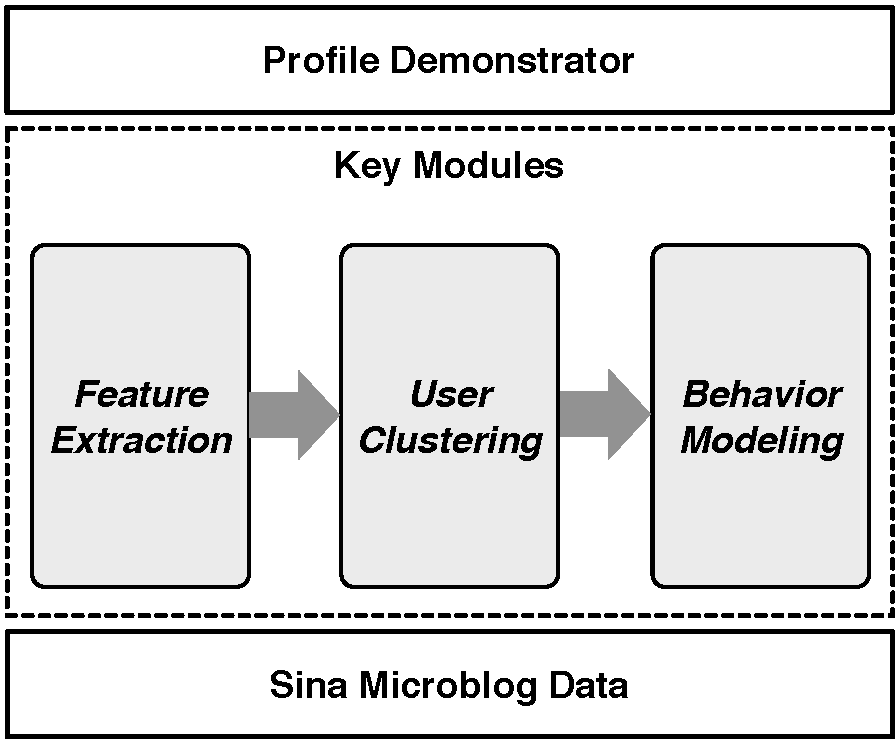
\includegraphics[width=.7\linewidth]{figures/architecture.pdf}
\caption{\sys{} Architecture}
\label{fig:framework}
\end{figure}


% #like and #comment are saved; could generalize \sys{} to model the liking behavior (among commented blogs)
\begin{comment}
\begin{figure}[!htb]
\centering
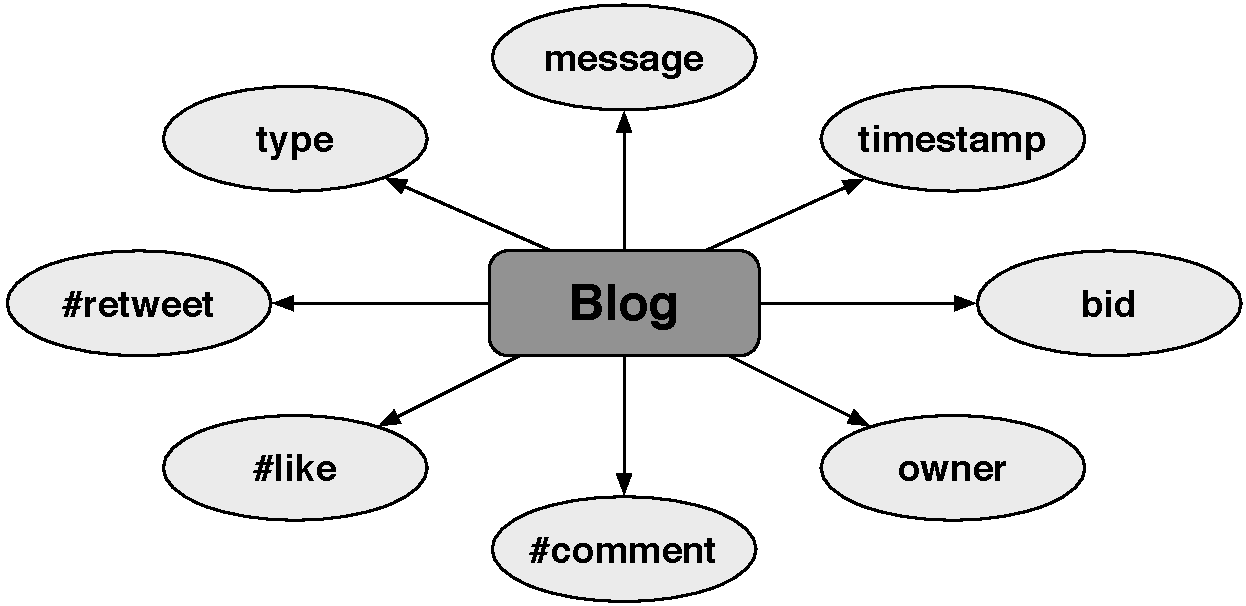
\includegraphics[width=.99\linewidth]{figures/microblog}
\caption{Blog Data in \sys{}}
\label{fig:blog}
\end{figure}
\end{comment}

\begin{comment}
\begin{figure}[!htb]
\centering
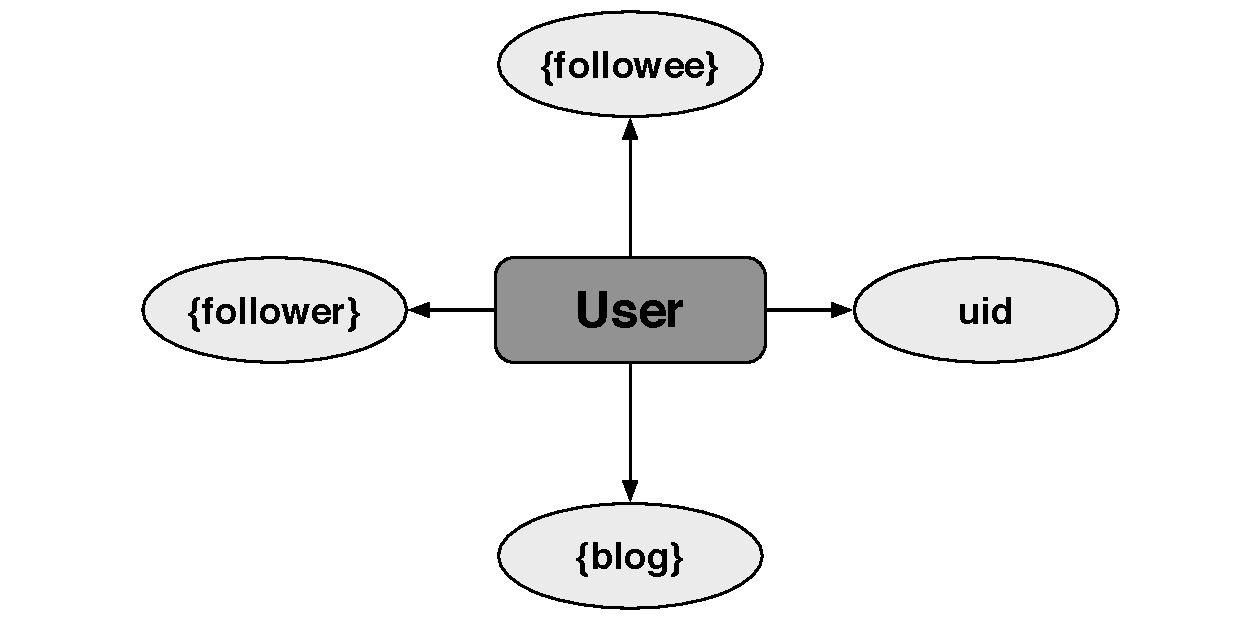
\includegraphics[width=.99\linewidth]{figures/user}
\caption{User Data in \sys{}}
\label{fig:user}
\end{figure}
\end{comment}


\stitle{Sina Microblog Data.} It is the data to be processed by \sys{}, i.e., data of microblogs and users, as shown in \textit{Definitions} \textit{\ref{def:blog}} and \textit{\ref{def:user}}.

\stitle{Key Modules.}
\sys{} consists of three key modules.
%\begin{enumerate}

	\stab(1)  Feature Extraction: By coalescing the microblog data, each user is depicted by a bunch of features, which are grouped into three categories. They are features of \textit{Basics} (e.g., the number of followers and followees), \textit{Behavior} (e.g., the frequency and the popular slots of \retg{}) and \textit{Interest} (e.g., the long-term/recent interests, as well as the explicit/implicit interests). These features are extracted from the stored data by Feature Extraction module and serve as the input of User Clustering module.
	
	\stab(2)  User Clustering: Providing the user-based features, User Clustering takes charge of the clustering task such that each user falls into a proper group.
	
	\stab(3)  Behavior Modeling: For each group obtained by User Clustering, Behavior Modeling employs both positive and negative samples (i.e., microblogs that were labeled with \retd{} and not \retd{}) to train a model, over which the testing of users' \retg{} behavior is performed.
%\end{enumerate}
	
\stitle{Profile Demonstrator.} At the top layer of \sys{}, it is the Profile Demonstrator for visualization.
%For the time being, Profile Demonstrator presents \tbc{}.



